\Chapter{Magyar felsőoktatási szabadságnyilvántartó szoftverszolgáltatás fejlesztése}

Célszoftver fejlesztése esetén a szoftver fejlesztést megelőzi egy kutatás és igény felmérés, ami során feltérképezzük a felhasználói igényeket, és az ezekhez tartozó elérhető kínálatot. Az igényeknek megfelelően pedig új hasznos funkciókat adunk a saját programunkhoz.

A felhasználók tökéletes forrást biztosítanak az ötletek és igények kialakításához, viszont ezeknek a megértéséhez, megvalósításához szükség van háttér ismeretekre is mint például jogszabályok és alap fogalmak. Amik alapján megtervezhető a program struktúrája, és működése is jobban leírható.

Miután megvan a szükséges tudás, a célnak megfelelően technológiai eszköztárat kell választanunk, valamint tudnunk kell milyen fejlesztési metodológiát alkalmazunk a feladatok és eredmények nyomon követésére. 

Ez a fejezet felvázolja, az elérhető lehetőségek hiányosságait a Magyar felsőoktatásban dolgozók mint felhasználók szempontjából, definiálja a témakörben használatos elméleti fogalmakat, valamint részletesen bemutatja a választott technológiai eszköztárat és folyamatokat.

\Section{Fogalmak, törvények, meghatározott feltételek}

Fontos, hogy tisztában legyünk a tervezés során számunkra lényeges meghatározásokkal, szabályokkal. A fejezet ezen részében a tervezés szempontjából szükséges, a munkatörvénykönyvében definiált fogalmakat, szabályozásokat mutatom be.

\subsection{Szabadság}

A szabadság olyan napok összessége, melyet a munkavállaló szerződésében foglalt munkanap helyett, munkahelyétől és a munkavégzéstől távol tölt. A tervezett szabadnapokat, a munkáltató felé, a munkavállalónak meghatározott idővel előre kell jelezni. Mind a két félre vonatkozó törvények, ész szabályozások akár évente változhatnak így követnünk kell az aktuális évben érvényes kiadásokat.

A szabadságnak két fajtája van:
\begin{itemize}
	\item \textbf{Fizetett\footnote{A dolgozat későbbi részében részletes bemutatásra kerül.}:} Szintén két részre bontható, munkanapnak minősül, szabályok alapján előre definiált, a munkavállaló pihenését és regenerálódását szolgálja. 
	\item \textbf{Fizetés nélküli:} A fizetett szabadságon felül igénybe vett szabadnapok, alapos indokkal vagy közös megegyezés esetén élhet vele a munkavállaló, ezekre a napokra nem köteles a munkáltató fizetést biztosítani. \cite{fizetesNelkuliSzabadsag}
\end{itemize}

\subsection{Fizetett szabadság}

A fizetett szabadság definíciója: 

"A szabadságnak a munkavállaló pihenését, regenerálódását szolgáló rendeltetéséből következik, hogy az alapvetően a ténylegesen munkában töltött idő után illeti meg a munkavállalót minden naptári évben. Mindazonáltal a törvény tényleges munkavégzés hiányában is munkában töltött – így szabadságra jogosító – időnek minősíti a következő időtartamokat:
\begin{itemize}
\item a munkaidő-beosztás alapján történő munkavégzési kötelezettség alóli mentesülés időtartama (ilyennek minősülnek például a pihenőnapok, pihenőidők vagy a rendkívüli munkavégzés ellenértékeként biztosított szabadidő),
\item a szabadság időtartama,
\item a szülési szabadság időtartama,
\item a gyermek gondozása céljából igénybe vett fizetés nélküli szabadság első hat hónapja,
\item a naptári évenként harminc napot meg nem haladó keresőképtelenség (a naptári évre eső egyes keresőképtelenségek tartamát össze kell számítani),
\item a tényleges önkéntes tartalékos katonai szolgálatteljesítés három hónapot meg nem haladó tartama,
\item a munkavégzés alóli mentesülésnek az 55. § (1) bekezdés b)–k) pontban meghatározott tartama (az emberi reprodukciós eljárással összefüggő, egészségügyi intézményben történő kezelés tartama; a kötelező orvosi vizsgálata tartama; a véradáshoz szükséges, legalább négy órás időtartam; a szoptató anyát megillető, a szoptatás első hat hónapjában naponta kétszer egy, ikergyermekek esetén kétszer két órás, a kilencedik hónap végéig naponta egy, ikergyermekek esetén naponta két órás időtartam; hozzátartozó halálakor két munkanap;" \cite{fizetettSzabadsag}
\end{itemize}

A meghatározás, továbbiakban kitér az éves szabadság keret összetételére mely szerint minden munkavállaló részére "alap és pótszabadságból áll"\cite{fizetettSzabadsag}.

\subsection{Alapszabadság}

Az alapszabadság, átlag munkavállaló esetén éves húsz napban van meghatározva. Ez bizonyos esetekben mint például, közalkalmazottak és oktatók eltérhetnek, de minden esetben meghaladják a korábban említett húsz napot.\footnote{Későbbi fejezetekben részletesebben tárgyalom ennek az eltérésnek a fontosságát.}\cite{fizetettSzabadsag} \cite{alapszabadsag}

\subsection{Pótszabadság}   
A pótszabadság több különböző feltételnek megfelelően jól definiált és körülhatárolt értékek összessége, amelyek lehetnek állandó tehát érvénybelépésüket követően folyamatosan minden évben jogosult rá a munkavállaló.
Valamint lehet eseti miszerint bizonyos életeseményekhez köthető, ideiglenes akár még korlátozott időtartamú felhasználhatóságról beszélhetünk.

A \aref{fig:potszab1} és \aref{fig:potszab2} ábrán láthatóak, a fajtái valamint az azokhoz tartozó munkanapban számolt értéke a 2013-as évben\cite{fizetettSzabadsag} \cite{alapszabadsag}.

\begin{figure}[h]
	\centering
	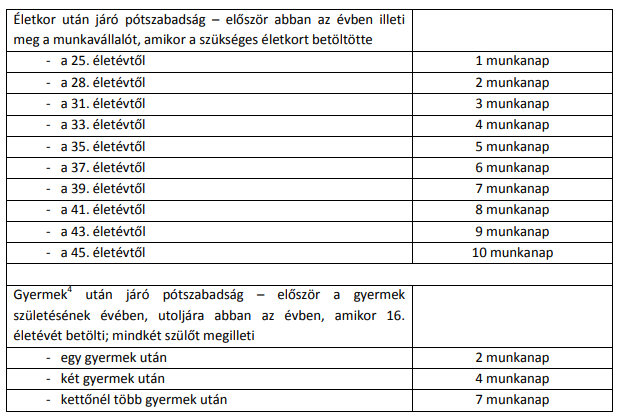
\includegraphics[scale=0.8]{images/potszabadsagok_1.png}
	\caption{Pótszabadságok típusai és értékei}
	\label{fig:potszab1}
\end{figure}

\begin{figure}[h]
	\centering
	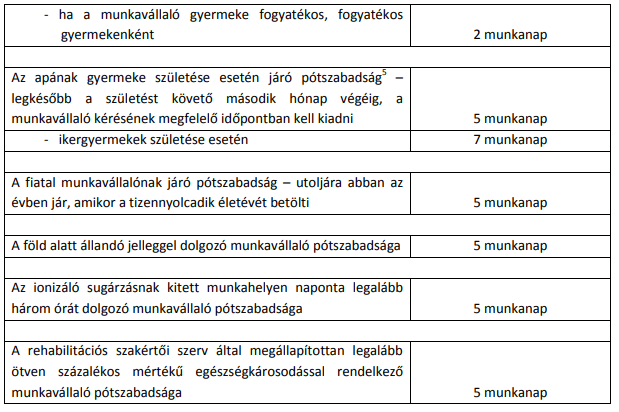
\includegraphics[scale= 0.8]{images/potszabadsagok_2.png}
	\caption{Pótszabadságok típusai és értékei}
	\label{fig:potszab2}
\end{figure}

\subsection{Közalkalmazottak szabadsága}

A közalkalmazottak szabadságolása nagyban eltér az átlag munkavállaló szabadságolásától. Alap szabadságuk fizetési osztálytól függően változhat, valamint nem teljesen ugyan azok a pótszabadságokkal kapcsolatos szabályok vonatkoznak rájuk mint egy átlag munkavállalóra.

"A közalkalmazottat
\begin{itemize}
	\item az „A”, „B”, „C” és „D” fizetési osztályban évi húsz munkanap,
	\item az „E”, „F”, „G”, „H”, „I”, „J” fizetési osztályban és a 79/C. §-ban említett munkakör betöltése esetén évi huszonegy munkanap
\end{itemize}

alapszabadság illeti meg."\cite{kozalkalmazottiSzabadsag}

\subsection{Időarányos szabadság}

"A munkavállalót a szabadság naptári évenként (tárgyév) illeti meg, ezért a részére járó szabadságnapok számát minden tárgyévben meg kell állapítani. Az ennek megfelelően meghatározott szabadság a munkavállalónak, ha munkajogviszonya a tárgyévben egészében nem áll fenn, azaz a naptári év közben létesül vagy szűnik meg, arányosan jár. " \cite{idoaranyosszabadsag}

Az éves szabadság megállapításakor tehát figyelembe kell vennünk, hogy a munkavállaló az adott évben ténylegesen mennyi munkanapot tölt alkalmazásban. Egy egyszerű matematikai képlet alkalmazásával számoljuk ki az alkalmazott éves szabadságát. 

Egy példán keresztül bemutatva a következőképp számoljuk egy munkavállaló időarányos szabadnapjait egy évre.

"A munkavállalót alapszabadságként 20 munkanap szabadság illeti meg naptári évenként. Ezen túlmenően az Mt. számos jogcímen (életkor alapján, 16 éven aluli gyermekekre tekintettel, speciális munkakörökben stb.) határoz meg pótszabadságokat, amelyek együttesen is megillethetik a munkavállalókat.

Az időarányosítás elvégzéséhez első lépésben meg kell állapítani a munkavállalót megillető szabadság mértékét. Ezt attól függetlenül munkanapban kell megtenni, hogy a munkáltató a szabadságot egyébként munkanapban vagy órában tartja nyilván.  Így például, egy harminchárom éves, két tizenhat év alatti gyermeket nevelő munkavállalót, aki állandó jelleggel föld alatt dolgozik, az alábbi jogcímeken illeti meg szabadság:

\begin{itemize}
	\item alapszabadság (20 munkanap)
	\item életkori pótszabadság (4 munkanap)
	\item gyermekek után járó pótszabadság (4 munkanap)
	\item föld alatti munkavégzés miatt (5 munkanap).
	\item föld alatti munkavégzés miatt (5 munkanap).
\end{itemize}

Azaz, a munkavállalónak mindösszesen 33 munkanap szabadsága van.

Az így megállapított összes szabadságot arányosítani kell, a munkaviszony év közben történő keletkezése, illetve megszűnése esetén. A fenti példában szereplő munkavállalót, amennyiben munkaviszonya 2016. július 1-jén fog elkezdődni (ekkor tárgyévben legfeljebb 184 napot fog munkaviszonyban állni) \( 33/365*184= 16,64 \) munkanap szabadság illetné meg.

Tekintettel arra, hogy az így kiszámított szabadság töredéknapot eredményez, alkalmazni kell az Mt. azon szabályát, hogy a fél napot elérő töredéknap egész napnak számít. Azaz, a munkavállalót mindösszesen 17 munkanap szabadság illeti meg 2016-ban."\cite{idoranyosSzamolasPelda}

Tehát az általános egyenlet a következő:
\begin{equation}\label{szabadság Számítás Tört Év esetén}
		\frac{MunkavallaloEvesSzabadsaga}{TargyEvNapokban*TargyEvbenHatralevoMunkanapok}=\lceil szabadsag \rceil
\end{equation}

\subsection{Szabadságok felhasználása}

Fontos tudni, hogy a munkavállaló nem rendelkezik teljes mértékben a számára meghatározott éves szabadság kerettel.

"A munkáltató évente hét munkanap szabadságot legfeljebb két részletben a munkavállaló kérésének megfelelő időpontban köteles kiadni azzal, hogy a munkavállalónak erre vonatkozó igényét legalább tizenöt nappal a szabadság kezdete előtt be kell jelentenie. A hét napos szabály jelentősége, hogy amennyiben a munkavállaló szabályszerűen bejelentette szabadságigényét, azt a munkáltató nem mérlegelheti.

Fontos, hogy ez a hét napos szabály a munkaviszony első három hónapjában nem köti a munkáltatót, azaz a munkaviszony első három hónapjában a munkavállaló a hét szabadnap általa meghatározott időpontban történő felhasználási jogával nem élhet. Ez utóbbi szabályt a legtöbbször – tévesen – úgy értelmezik, hogy próbaidő alatt, illetve az első három hónapban nem lehet szabadságra menni. [...]

Fontos kötelezettsége a munkáltatónak, hogy a szabadságot úgy kell kiadnia, hogy a munkavállaló naptári évenként egy alkalommal, legalább tizennégy egybefüggő napra mentesüljön a munkavégzési és rendelkezésre állási kötelezettsége alól. Ettől a szabálytól azonban a felek eltérhetnek.

A tizennégy napos szabály tekintetében – a szabadságként kiadott napon túl – a heti pihenőnap (heti pihenőidő), a munkaszüneti nap és az egyenlőtlen munkaidő-beosztás szerinti szabadnap vehető figyelembe." \cite{szabadsagFelhasznalasa}

\Section{Jelenleg elérhető megoldások}

A rengeteg szabályozásból, csak párat kiemelve jól látszik, hogy az automatizáláshoz szükséges számítások nem túl bonyolultak. A törvények összetett struktúrája, viszont országonként eltér, sőt a munkavállalókra különböző jogszabályok vonatkoznak amennyiben azok közalkalmazottak. Ezen információk fényében a vizsgálható, az elérhető megoldások amiket a jelenlegi piac kínál.

\subsection{Nemzetközi szoftverek}

Szinte számtalan applikáció elérhető a nemzetközi piacon, és ezek mindegyike minőségi szolgáltatás nyújt egy modern és könnyen kezelhető design keretében. Összességében mindegyikről elmondható, hogy ezek a szolgáltatások havidíjas előfizetéssel, működnek és többnyire tartozik hozzájuk egy profi támogatói csoport is akik mind konfigurálás, mind felhasználói problémák esetén is elérhetőek. 

Továbbá az is jól látszik, hogy több országban jelen vannak így nem csak az általános pótszabadságokat tudjuk ezeken keresztül kezelni, de akár saját személyre szabott típust is definiálhatunk.

Hátrányuk, viszont nem csak a havi díjban megszabott ár hanem az ehhez tartozó felhasználói létszám keret vagy akár a csomagban definiált funkció korlátozás is. Látható még, hogy ezek az alkalmazások vagy csak egy funkcióként kezelik a szabadság nyilvántartást, vagy egy több szolgáltatásból álló egység külön része ami arra enged következtetni, hogy bár külön álló program ként is funkcionál, bizonyos előnyök csak a többi testvér szolgáltatással együtt használhatóak.

Végül láthatjuk, hogy egyik alkalmazás bemutató anyaga sem tér ki a közalkalmazottakra, így azt feltételezhetjük, hogy ezek a szolgáltatások nincsenek felkészítve a közalkalmazotti különbségekre.

A \ref{tab:nemzetközi programok} \texttt{Nemzetközi programok összehasonlítása} táblázatban látható néhány elérhető megoldás.

\begin{table}[h]
	\centering
	\caption{Nemzetközi programok összehasonlítása.}
	\label{tab:nemzetközi programok}
	\begin{tabular}{|>{\centering\arraybackslash}m{3cm}|>{\centering\arraybackslash}m{5.5cm}|>{\centering\arraybackslash}m{5.5cm}|}
		\hline
		Termék megnevezése & Tulajdonságok & Csomag árak \\
		\hline
		freshworks, freshteam, Time Off\cite{freshworkswebsite} & Teljes körű HR szolgáltatás, felhasználó adatbázis, munkaidő követés, alapvető vagy akár bonyolult szabadság kezelés   & Ingyenes(nem tartalmaz egyéni szabadság kezelési lehetőséget), 75\$ - 250\$/hó/50 felhasználó \\
		\hline
		Leave Dates\cite{leavedateswebsite} & Idő menedzsment, szabadság kezelés  & Ingyenes 5 felhasználóig, 1\$/hó \\
		\hline
		AnnualLeave\cite{annualleavewebsite} & Idő menedzsment, szabadság kezelés  & Árajánlat kérés alapján, elérhető kalkulátoruk szerint 22\$/hó(20 főre) \\
		\hline
		Calamari\cite{calamariwebsite} & Szabadság kezelés, felső vezetői jóváhagyási rendszer, nemzetközi naptárak  & Felhasználók mennyiségétől függ 25\$/hó(20 főre) \\
		\hline
	\end{tabular}
\end{table}

\subsection{Magyar fejlesztésű programok}

A piacon található Magyar eredetű megoldások többsége valamiért még mindig az összetett excel táblázatokon alapul, amikben bonyolult függvények és macro programozással valósítják meg a nyomon követést.

Ezeknek a megoldásoknak a legnagyobb hibája a nehezen megoldható konkurens kezelés valamint, a felhasználó számítógépével való szoros függőség. Mindezek mellett sérülékeny, az óvatlan szerkesztés és mentés esetén könnyen az egész táblázat hamis adatokat mutathat. Esetleges hiba bekövetkeztével a pótlásuk nehézkes, szinte lehetetlen.

Fellelhetőek itt is kifejezetten a témával kapcsolatos szoftverek vagy akár teljes szolgáltatások is. Ezek a lehetőségek többnyire komplex rendszerek több, esetenként akár felesleges funkcióval.

A \aref{tab:magyar programok} \texttt{Magyar megoldások összehasonlítása} táblázatban látható néhány elérhető megoldás.

\begin{table}[h]
	\centering
	\caption{Magyar megoldások összehasonlítása}
	\label{tab:magyar programok}
	\begin{tabular}{|>{\centering\arraybackslash}m{3cm}|>{\centering\arraybackslash}m{5.5cm}|>{\centering\arraybackslash}m{5.5cm}|}
		\hline
		Termék megnevezése & Tulajdonságok & Csomag árak \\
		\hline
		Szabadság tervező és nyilvántartó\cite{hatekonysagwebsite} & Szabadság nyilvántartó excel táblázat   & 6 felhasználóig ingyenes, 21-50 felhasználóig 21.000 Ft + ÁFA/hó \\
		\hline
		excelmester\cite{excelmestergwebsite} & Szabadság nyilvántartó excel táblázat  & Ingyenes\\
		\hline
		HRmaster\cite{hrmasterwebsite} & Összetett erőforrás menedzser szoftver  & Árajánlat kérés alapján \\
		\hline
		PREDOR\cite{predorwebsite} & Munkaidő nyilvántartó és biztonsági rendszer  & Árajánlat kérés alapján \\
		\hline
	\end{tabular}
\end{table}

\Section{Fejlesztési lehetőségek}

Az elérhető megoldásokat összegezve láthatjuk, hogy többségük a munkavállaló szempontjából könnyen használható, mégis számunkra kényelmetlen konfigurációs problémákat vethet fel, amennyiben alkalmazottainkra eltérő szabályokat kell alkalmaznunk. Megfigyelhetjük azt is, hogy az összetettebb statisztikai lehetőségeket biztosító alkalmazások meglehetősen költségesek egy felsőoktatási intézmény számára, és akár megannyi számunkra kevésbé hasznos később kihasználatlan funkciót is tartalmazhatnak.

Továbbá általánosan elmondható a promóciós anyagok alapján, hogy az automatizált működés nincs megvalósítva.
\vskip 0.2in
Amennyiben leszűkítjük a felhasználók körét a felsőoktatásban dolgozó oktatókra és az azokkal együtt, tevékenykedő adminisztrátorokra láthatóvá válik, hogy bár az egyetemek használnak központi alkalmazásokat de egy-egy intézetben már megjelennek az eltérő szabályok. Egy egységben egyszerre vannak jelen normál, és közalkalmazotti jogviszonnyal rendelkező munkavállalók is, ezen felül szervezeti egységenként az-az tanszékenként, intézetenként a szabadságok jóváhagyásáért az adott egység vezetője a felelős. Felelősségi körébe viszont beletartozik egy éves szabadságolási terv előállítása is amelynek be kell tartania a szabadság felhasználásával kapcsolatos jogszabályokat is. Az említett tervezetet valamint időközi statisztikákat jelenleg manuálisan állítják össze és továbbítják a központi rendszerbe.
\vskip 0.2in
Mindent egybevetve a piacon fellelhető applikációk több extra funkciótól mentes de mégis számunkra specifikus alkalmazást hozhatunk létre a következő működések megvalósításával:

\begin{itemize}
	\item A felhasználó egyedi szabadságolással kapcsolatos adatait tartalmazó adatbázis
	\item A Magyar törvényekre specifikus szabadság típusoknak megfelelő konfigurálási lehetőség
	\item Dinamikus alkalmazhatóság, eltérő alkalmazotti jogkörök esetén.
	\item Automatikus kalkuláció teljes és részleges tárgy év esetén.
	\item Felettesi jóváhagyás támogatása.
	\item Éves szabadságolási tervező / Automatikus generálás.
	\item Tetszőleges statisztikák lekérdezése.
	\item Felhasználó jól átlátható, követhető szabadnap menedzsmentje.
\end{itemize}

\Section{Technológiai eszköztár}

A konkrét tervezési lépések megkezdése előtt rendkívül fontos az alkalmazásunk számára megfelelő technológiai hátteret biztosítani.

Választásunk során nem elég figyelembe venni mi az amit kezelni tudunk, fontos előretekintően lehetőleg minél modernebb technológiákat alkalmazni amik nagyban könnyíthetik bizonyos műveletek elvégzését a megvalósítás során, valamint lehetőséget nyújtanak a későbbi fejlesztés egyszerűsítésére is.

Ellenben nem érdemes kiforratlan kezdetleges de divatos eszközökhöz sem, hozzákötni magunkat!

\subsection{Verziókezelés és Verziókezelő rendszerek}

"Verziókezelés alatt több verzióval rendelkező adatok kezelését értjük. Leggyakrabban a mérnöki tudományokban és a szoftverfejlesztésben használnak verziókezelő rendszereket fejlesztés alatt álló dokumentumok, tervek, forráskódok és egyéb olyan adatok verzióinak kezelésére, amelyeken több ember dolgozik egyidejűleg. Az egyes változtatásokat verziószámokkal vagy verzióbetűkkel követik nyomon."\cite{verziokezeles}

Lényeges pontja a fejlesztésnek, hogy a forráskód, ne csak a saját gépünkön legyen elérhető, amennyiben csapatban dolgozunk ez a szempont kiemelten fontos lehet, nagyban könnyítheti a mindennapokat, ha egymástól függetlenül könnyen tudunk változtatásokat eszközölni a kódbázison.

Ezeknek a rendszereknek a gyakorlati haszna túlmutat a forráskód konkurens kezelhetőségén, stabil verziók esetén szerves részét képezik mindennapi használatban lévő úgynevezett "éles" vagy "production" környezetbe való kitelepítését.

\paragraph{SVN}

"A Subversion (SVN) egy verziókezelő rendszer, melyet a CollabNet Inc. indított 2000-ben. Fájlok aktuális verzióinak és történeteinek kezelésére használják, mint például forráskódok, weboldalak és dokumentációk. A célja, hogy a legkompatibilisebb utódja legyen a széles körben használt Concurrent Versions System (CVS)-nek."\cite{svn}

Az SVN alapú rendszerek jól használhatóak a lineáris fejlesztésben, de agilis fejlesztési modell esetén sokkal nem elég rugalmasak és nehezebben kezelhetőek.

Korábban a legnépszerűbb használatban lévő rendszer, mai napig megtalálható a piacon, viszont a modernebb koncepciók elterjedésével egyre ritkábban találkozhatunk SVN-ben kezelt kódbázissal.

\paragraph{Git}

"A Git egy nyílt forráskódú, elosztott verziókezelő szoftver, vagy másképpen egy szoftverforráskód-kezelő rendszer, amely a sebességre helyezi a hangsúlyt. A Gitet eredetileg Linus Torvalds fejlesztette ki a Linux kernel fejlesztéséhez. Minden Git munkamásolat egy teljes értékű repository teljes verziótörténettel és teljes revíziókövetési lehetőséggel, amely nem függ a hálózat elérésétől vagy központi szervertől."\cite{git}

Gyors és skálázható rendszer, könnyen és dinamikusan kezelhető kis és nagy létszámú csapatok esetén is. Gyorsan tanulható és könnyen átlátható, a lokális repository már kezdő fejlesztőként is segíti és gyorsítja az egyes fejlesztési műveleteket. Megfelelő beállítások, használat esetén a központi repository stabil ága jól védett, ezáltal folyamatos lehetőséget biztosít az általunk fejlesztett szoftver legfrissebb működő állapotának az "éles" végfelhasználók számára elérhető környezetre való kitelepítését.

Jelenleg széles-körben használt, elterjedt és népszerű technológia. A megvalósítás során én is ezt a technológiát használtam fel.

\subsection{Programozási nyelvek}

Webfejlesztés esetén több meghatározó területet definiálhatunk, de ezek közül is leginkább a Backend az-az háttér rendszeri fejlesztés, valamint a Frontend tehát a felhasználói felület és megjelenítés fejlesztés amit főbb tagolásnak nevezhetünk. Ezek a területek funkciójukban és feladatkörükben elválaszthatóak, többnyire külön micro alkalmazások ként működnek, így fontos megemlíteni, hogy bár minden esetben egymással kommunikálnak, többnyire egymástól független programozási nyelveken íródnak.

Mind a két területről elmondható, hogy nagy választékkal rendelkeznek nyelvek területén, ezek folyamatosan megújuló megoldások ezért ezen a területen kiemelten fontos, hogy körültekintően válasszunk! Egy friss és dinamikus megoldásokat kínáló nyelv gyakran lehet kiforratlan és kevésbé előnyös a későbbi fejlesztések során a jól bevált már ismert nyelvekkel szemben.

\paragraph{Háttérrendszer, Backend}

Ezen a területen bár mostanában kezd elterjedni a node.js, mégis a C\# és Java nyelveket mondhatjuk meghatározónak. Bár mind a C\# is elismert és több helyen használt, mégis mondhatni jelenleg a Webfejlesztés piacán a Java az elterjedtebb és támogatottabb nyelv.

\subparagraph{Java}

"A Java általános célú, objektumorientált programozási nyelv, amelyet a Sun Microsystems fejlesztett a ’90-es évek elejétől kezdve egészen 2009-ig, amikor a céget felvásárolta az Oracle.

A Java alkalmazásokat jellemzően bájtkód formátumra alakítják, de közvetlenül natív (gépi) kód is készíthető Java forráskódból. A bájtkód futtatása a Java virtuális géppel történik, ami vagy interpretálja a bájtkódot, vagy natív gépi kódot készít belőle, és azt futtatja az adott operációs rendszeren. Létezik közvetlenül Java bájtkódot futtató hardver is, az úgynevezett Java processzor.

A Java nyelv a szintaxisát főleg a C és a C++ nyelvektől örökölte, viszont sokkal egyszerűbb objektummodellel rendelkezik, mint a C++. A JavaScript szintaxisa és neve hasonló ugyan a Java-hoz, de a két nyelv nem áll olyan szoros rokonságban, mint azt ezekből a hasonlóságokból gondolhatnánk. [...]

A nyelv első tulajdonsága, az objektumorientáltság („OO”), a programozási stílusra és a nyelv struktúrájára utal. Az OO fontos szempontja, hogy a szoftvert „dolgok” (objektumok) alapján csoportosítja, nem az elvégzett feladatok a fő szempont. Ennek alapja, hogy az előbbi sokkal kevesebbet változik, mint az utóbbi, így az objektumok (az adatokat tartalmazó entitások) jobb alapot biztosítanak egy szoftverrendszer megtervezéséhez. A cél az volt, hogy nagy fejlesztési projekteket könnyebben lehessen kezelni, így csökken az elhibázott projektek száma. [...]

A Java legfontosabb része a Java virtuális gép (Java Virtual Machine – JVM). A JVM mindenütt jelen van (szinte mindenféle berendezés, chip és szoftvercsomag tartalmazza), így a nyelv középszintként és platformként egyaránt működik. Ugyanakkor a nyelv „platformfüggetlen” is, mert a Java virtuális gépek interpretálják a szabványos Java bájtkódot. Ez azt jelenti, hogy egy PC-n megírt Java program minimális módosítás után ugyanúgy fog futni egy javás telefonon is. Innen jön az írd meg egyszer, futtasd bárhol kifejezés. Ez jelentős költségcsökkenést eredményez, mert a kódot csak egyszer kell megírni."\cite{java}

A megvalósítás során Java 11-es verziót használtam, melyben elérhetőek a lambda és stream nyelvi elemek.

\paragraph{Megjelenítés, Frontend}

A megjelenítési réteg webapplikációk esetén többnyire három fő részből áll. A HTML leírónyelveben íródó struktúra adja az oldalak felépítését, vázát. Ezt kiegészíti egy másik leíró nyelv a CSS ami minden esetben a megjelenő designért felelős. Valamint ide tartoznak még a különböző script nyelvek mint a javascript amelyek az böngészőben futó logikáért felelősek.
\vskip 0.2in
Java nyelv esetén beszélhetünk még a JSP technológiáról ami az említett frontend technológiákat ötvözte valamint lehetővé tette, hogy Java kódot építsünk be HTML-be. Ezzel elértük, hogy az alkalmazásunk szerves része legyen egy általunk generált megjelenés is. 

A mára elavultnak számító JSP technológiát egyszerűbb esetekben a hasonló működési elven alapuló szerver oldalon generált megjelenést biztosító Java template engine-ek váltották fel több helyen. Használatukban igen hasonlóak az elődjükhöz, viszont a különböző Java logikák mint az if vagy a for használata sokkal egyszerűbb és átláthatóbb. Az egyik legnépszerűbb alkalmazás ezen a téren a Thymleaf. 

\vskip 0.2in
A legmodernebb megoldás jelenleg az Angular logikával megvalósított megjelenítés. Ezen esetben is jelen van a HTML, valamint a CSS viszont az oldalunk tartalmát és akár megjelenítését is tudjuk változtatni akár csak a sima javascript esetén. Ez az elképzelés viszont objectum orientált alapokra helyezi a frontend fejlesztést, valamint saját különálló programként tekint a megjelenítési réteg kódbázisára. 

Tehát ebben az esetben arról beszélhetünk, hogy önállóan is futtatható a programunk megjelenítési rétege, így az a hátétrendszertől elkülönítve fejleszthető a két alkalmazás. Csupán kommunikációs kapcsolat van köztük így amennyiben arra igény van a megjelenítés, valamint a szerver oldali logika egymástól függetlenül cserélhető is.

\vskip 0.2in
Itt érdemes még megemlíteni az előre definiált designt biztosító Bootstrap szolgáltatást is, ami lehetővé teszi, hogy a megjelenítést gyorsan felépítsük már létező CSS elemekkel.

\subsection{Szoftver menedzsment eszköz}

Mivel meglehetősen időigényes akár a mindennapi fejlesztés terén az alkalmazásunk futtatására különféle parancsok megfelelő sorozatát kiadni, így igény keletkezett az automatizálható szoftver menedzsment eszközökre. Az egyik ilyen legelterjedtebb az Apache Ant volt eleinte. Viszont mára sokkal ismertebb és elterjedtebb a szintén Apache fejlesztésű Maven használata.

\paragraph{Maven} "Az Apache Maven (röviden Maven) egy szoftver, amelyet szoftverprojektek menedzselésére és a build folyamat automatizálására lehet használni. Jason van Zyl készítette 2002-ben. Funkcionalitásában hasonlít az Apache Ant eszközhöz (és némi hasonlóságot mutat a PHP-s PEAR-rel és a perles CPAN-nal, de egyszerűbb és XML-alapú a konfigurációs modellje). A projektet az Apache Software Foundation hosztolja, ahol korábban a Jakarta Projekt részeként működött.

A Maven bevezeti a POM, azaz a Projekt Objektummodell (angolul: Project Object Model) fogalmát. Egy POM egy buildelendő projektet ír le és annak függőségeit. Az egyes lépéseket céloknak, angolul goal-oknak nevezik. Vannak előre definiált célok a tipikus feladatokra, mint például a kód fordítása és csomagolása, de a felhasználónak lehetősége van saját célokat is definiálni a projektspecifikus lépések végrehajtására.

A Maven hálózatképes, tehát szükség esetén dinamikusan is le tud tölteni komponenseket. Repository névvel illetik a különböző hosztok fájlrendszereinek azon mappáit, ahol a letölthető komponensek találhatók. A Maven nem csak a repository-kból való letöltést támogatja, hanem a készült szoftvercsomag feltöltését is. Ezzel az automatizálható le- és feltöltési mechanizmussal a Maven de facto szabványt próbál teremteni, de elég lassan fogadja el a Java közösség.

A Maven plugin alapú architektúrája lehetővé teszi tetszőleges parancssorból vezérelhető alkalmazás használatát. Ez elméletileg lehetővé teszi tetszőleges programnyelvekhez való pluginek készítését, de a gyakorlatban minimális mennyiségű nem javás plugin készült."\cite{maven}

\vskip 0.2in
Fontos megemlíteni, hogy bár a Maven jelenleg a legelterjedtebb manapság egyre népszerűbb a Gradle is, ami átláthatóbb és dinamikusabban konfigurálható, mégis egyetlen hátránya van ami miatt kevesebben használják és ez csupán az, hogy kevésbé ismert.

\subsection{Keretrendszerek}

Habár csak és kizárólag Java nyelv használatával is képesek vagyunk megvalósítani egy számunkra megfelelő alkalmazást, mégis érdemes megkönnyíteni a saját dolgunkat különböző keretrendszerek használatával. Korábban ilyen volt a Java EJB, mára viszont sokkal kifinomultabb megoldások léteznek, a webalkalmazások terén az egyik legismertebb a Spring valamint az arra épülő Spring-boot.

\paragraph{Spring}

"A Spring egy nyílt forráskódú, inversion of controlt megvalósító Java alkalmazás keretrendszer.
A Spring keretrendszer több önálló modulból épül fel, amelyek az alábbi szolgáltatásokat nyújtják a fejlesztők számára:

\begin{itemize}
	\item Inversion of control konténer: a Java objektumok életciklusának kezelése és az alkalmazás-komponensek testreszabása.
	\item Aspektus orientált programozási paradigma követésének lehetősége.
	\item Adatelérés: lehetőség van relációs adatbázis-kezelő rendszerek JDBC segítségével történő elérésre, és objektum-relációs leképzések, NoSQL integrálására.
	\item Tranzakciókezelés: többféle tranzakció kezelő API-t tartalmaz.
	\item Modell-nézet-vezérlő szabvány: egy HTTP- és servlet alapú keretrendszer segítségével valósítható meg, amelyet arra fejlesztettek ki, hogy bővíthetők és személyre szabhatóak legyenek a webszolgáltatások
	\item Távoli eljáráshívás kezelő keretrendszer: biztosítja a RPC alapú, hálózaton keresztül történő Java objektum importokat és exportokat. További támogatást nyújt a RMI, a CORBA és HTTP alapú protokollok \item használatára, beleértve a webszolgáltatásokat (SOAP) is.
	\item Kötegelési eljárás támogatása.
	\item Azonosítás és azonosságkezelés: biztonsági folyamatok konfigurálása, melyet a Spring projekthez tartozó, Spring Security alprojekt tesz lehetővé a különféle protokollok és módszerek biztosításával.
	\item Üzenetkezelés: a JMS API-n keresztül történő általános üzenetkezelés továbbfejlesztése érhető el.
	\item Tesztelés: segítséget nyújt a unit- és az integrációs teszt írására."\cite{spring}
\end{itemize}

\subparagraph{Inversion of control (IoC) avagy a kontroll megfordítása} "főleg objektumorientált programozási nyelvekben használt technika a komponensek összeillesztésére, konfigurálására és kezelésére.

A technika lényege, hogy a komponenskezelést (pl. létrehozást, példányosítást, paraméterezést, megszüntetést, metódus hívás) kiemeljük a programkódból, és általában egy külső keretrendszerre bízzuk, mint pl. a Spring.

Célja a modularitás növelése és bővíthetővé tétele. Az objektumorientáltság nem feltétel. A kifejezést Robert C. Martin és Martin Fowler népszerűsítette.

Egy rokon minta a függőség befecskendezése, ami a függőségeket megosztott absztrakcióval kezeli a felső és az alsó rétegek között. Kapcsolódik az eseményvezérelt programozáshoz is, mert azt gyakran a kontroll megfordításával valósítják meg. A felhasználó kódja csak az eseményeket dolgozza fel, míg az eseményciklus és az események, üzenetek közvetítése a keretrendszerre vagy a futtató környezetre van bízva."\cite{ioc}

\subparagraph{Spring konfigurálása}

Ahhoz, hogy az általunk megírt osztály a keretrendszerben létezzen, konfigurálnunk kell belőle egy példányt amit fel tud dolgozni és a saját kontextusába be tud illeszteni. Ennek az úgynevezett bean definíciónak három módja van. XML, Java valamint annotáció alapú konfigurációból választhatunk, de akár keverhetjük is őket ami nehezíti a kód megértését így semmiféleképp nem ajánlott. Mindegyiknek megvan természetesen a maga előnye és hátránya. Csak rajtunk múlik melyiket használjuk de fontos, hogy lehetőleg maradjunk egy félénél és legyen konzisztens a kódunk.

\paragraph{Spring-boot}

Egy natív Spring alapú szolgáltatás melynek lényege, hogy gyorsan és még egyszerűbben tudjunk önálló webalkalmazásokat létrehozni. Amíg az egyszerű Spring esetén az összes elemet nekünk kell összerakni és bekonfigurálni, a boot esetén előre definiált egységeket használunk ami egy kezdetleges konfigurációval rögtön futtatható programot biztosít számunkra.

Továbbá ezen külső könyvtárak és megvalósítások újra konfigurálása is sokkal egyszerűbb.

Tartalmaz előre meghatározott annotációkat amik használatával másodpercek alatt hozhatunk létre a keretrendszer kontextusában létező osztályokat.  

\subsection{Adatbázis, Verzió kezelt adatbázis, ORM}

Napjainkban egyre több típusú adatbázis létezik, és mindegyiknek megvan a leghasznosabb felhasználási területe, már nem csak a jól ismert SQL típusok érhetőek el de megjelent a NoSQL valamint sok más koncepció alapján működő lehetőség is.

A megvalósítás szempontjából szinte tökéletesen megfelel a mindenki által ismert SQL típus, ez egy igen széles-körben elterjedt és alkalmazott adatbázis.

\paragraph{Liquibase} "egy ingyenes, nyílt forráskódú, adatbázisfüggetlen változáskövető eszköz, ami jól használható az elterjedt verziókövető eszközökkel. Lényege, hogy a szükséges adatbázismódosításokat nem közvetlenül az adatbázison hajtjuk végre, hanem minden változást struktúrált módon, egy ún. changelog fájlban tartunk nyilván. Ezt a changelog fájlt aztán a Liquibase parancssoros alkalmazás segítségével vagy kódból, a Liquibase Java API-val tudjuk érvényesíteni. Ennek használata a következő előnyökkel jár:

\begin{itemize}
	\item a changelog fájl feltölthető verziókövetőbe, ezáltal megvalósíthatjuk adatbázisunk verziókövetését;
	\item a Liquibase számon tartja, hogy mely változások kerültek korábban már érvényesítésre adatbázisunkon, és csak a szükségeseket futtatja." \cite{liquibase}
\end{itemize}

\paragraph{Objektum-relációs leképzés(ORM)}
"Az objektum-relációs leképzés (angolul \newline Object-Relational Mapping) egy programozási technika adatok konvertálására nem kompatibilis típusos rendszerek és objektumorientált programozási nyelvek között. Lényegében egy „virtuális objektum-adatbázist” hoz létre, amit a programozási nyelvben használhatunk."\cite{orm}

Egyik legismertebb megvalósítása a JPA, ami nem csak a részét képezi a spring-bootnak, hanem saját ORM rendszert épít rá Spring Data néven.

\subsection{Szoftver architektúra}

"A modell-nézet-vezérlő (MNV) (angolul model-view-controller) a szoftvertervezésben használatos programtervezési minta. Összetett, sok adatot a felhasználó elé táró számítógépes alkalmazásokban gyakori fejlesztői kívánalom az adathoz (modell) és a felhasználói felülethez (nézet) tartozó dolgok szétválasztása, hogy a felhasználói felület ne befolyásolja az adatkezelést, és az adatok átszervezhetők legyenek a felhasználói felület változtatása nélkül. A modell-nézet-vezérlő ezt úgy éri el, hogy elkülöníti az adatok elérését és az üzleti logikát az adatok megjelenítésétől és a felhasználói interakciótól egy közbülső összetevő, a vezérlő bevezetésével.

Hagyományosan asztali felhasználói felületekhez használt, de manapság már webalkalmazásokhoz is népszerűvé vált. Népszerű programozási nyelvek mint a JavaScript, Python, Ruby, PHP, Java, C\# és Swift már külön telepítés szükségessége nélkül rendelkeznek MNV keretrendszerekkel web- és mobilalkalmazások fejlesztésére."\cite{mvc}

\begin{figure}[h]
	\centering
	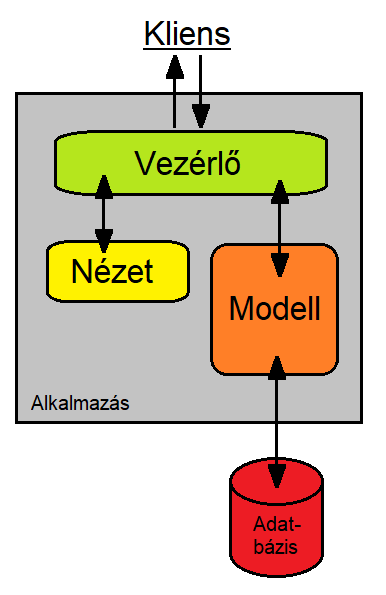
\includegraphics[scale= 0.8]{images/MNV-reprezentáció.png}
	\caption{MNV reprezentációja}
	\label{fig:mnv}
\end{figure}

Az MNV egy összetettebb változata  a több szintű architektúra amiben a korábban említett három rétegen felül saját rétegeket definiálunk és azok között belső transzformációkkal továbbítjuk az adatokat. Ilyen további rétegek lehetnek az Adat továbbítóréteg(DTO), a tartomány réteg (Domain) valamint az adat hozzáférési réteg (dal).

\vskip 0.2in
A többszintű alkalmazás architektúrák könnyebben átalakíthatóak Microservice architektúrákká, melyek fejlesztése és üzemeltetése egyszerűbb, költséghatékonyabb és stabilabb. 

\subsection{Tesztelés, Tiszta kód}

A fejlesztési folyamatok során elengedhetetlen, hogy folyamatosan kipróbáljuk és ellenőrizzük az általunk írt logikát. Ezeket az ellenőrzési folyamatokat nevezzük tesztelésnek.

A felületen történő funkcionális teszttől egészen a legapróbb kódsorig rengeteg lehetőségünk van a programunkat különböző tesztek alá vetni, hogy ténylegesen az elvárt működésnek megfelelően viselkedjen a szoftverünk.
Ezekhez támogatást nyújt számunkra a már említett Maven, valamint a Spring keretrendszer is. 

Különböző tesztelést segítő megoldások léteznek ilyen például a JUnit4, JUnit5 valamint a TestNG is, hogy  megtudjuk határozni a tesztek hatáskörét és garantáljuk egymástól való függetlenségüket, valamint, hogy meghatározzuk külső függőségek visszatérési értékét objectum utánzó objectumokat más néven Mock-okat használunk.

\paragraph{Egységtesztelés} "A számítógép-programozásban az egységtesztelés a szoftvertesztelésnek egy olyan módszere, amelynek során a forráskód egységeit (egy vagy több számítógépes program modul készletet) a kapcsolódó vezérlő adatokkal, a felhasználási-és a működtető eljárásokkal együtt tesztelik annak meghatározására, hogy azok elérik-e kitűzött céljukat."\cite{unittest}

Egység tesztelés során fontos meghatároznunk, mi az a legkisebb egység amit tesztelünk, általános megállapodás szokott lenni, hogy egy függvényt tekintünk tesztelendő egységnek. További megállapodás, hogy csak publikus elérésű függvényekre írunk tesztet, viszont a vélemények sokszor eltérnek a tesztesetek számát illetően. Vannak nézetek ami szerint minden lehetséges esetet le kell fedni, de a gyakorlatban legtöbbször csak az elvárt működést valamint a logika különböző agait szokás lefedni.

\paragraph{Manuális tesztelés}

Ahhoz, hogy az elvárt működést teljesen le tudjuk ellenőrizni, működés közben teszt adatok segítségével úgymond felhasználóként kipróbáljuk a funkciókat a felületen keresztül. Amennyiben csak háttérrendszerrel rendelkezünk ez a tesztelés továbbra is alkalmazható, a korábban már tárgyalt MNV modell miatt. A vezérlőt közvetlenül meg tudjuk hívni szimulálva ezzel a megjelenítési rétegtől érkező kérést, a szerver oldali alkalmazás pedig kiszolgálja azt egy JSON válasszal.

Ennek vizualizációjára szolgál a swagger-UI vagy más neven OpenAPI eszköz.\footnote{A dolgozat későbbi részében részletes bemutatásra kerül.}

\subparagraph{Tiszta kód}

Fontos megemlíteni, hogy a tesztek olvashatósága és egyszerűsége érdekében jól tagolt olvasható kódot kell produkálnia a fejlesztőnek. Ehhez szükség van előre definiált mérőszámokra mint például sorok hossza, függvények sorszáma, ciklomatikus komplexitás.

A nehezen olvasható és tesztelhető kódok, nagyobb valószínűséggel tartalmaznak hibát és szinte biztos, hogy újraírásra szorulnak.

A tiszta kód szabályai mindig a fejlesztőcsoport megegyezése alapján történnek, a szabályok betartása viszont nagyban könnyíti a későbbi fejlesztést. A megalkotásukhoz kiváló útmutató Robert C. martin, Clean Code : A Handbook of Agile Software Craftsmanship\cite{cleanCode} című könyve!

\subsection{Folyamatos integráció/Folyamatos szállítás (CI/CD)}

"A folyamatos integráció olyan fejlesztési gyakorlat, amelyben a fejlesztők a kódot naponta többször egy közös felületen integrálják, egyeztetik. Így a kisebb változtatások is gyorsan elérhetővé válnak a csapat többi tagja számára. Az integrálást követően minden új kódrészlet ellenőrzésre kerül, amely lehetővé teszi a fejlesztők számára, hogy korán felismerjék a problémákat és még az elején javítsák azokat, így időt nyerve és minimalizálva a javítandó kódok mennyiségét.

A folyamatos szállítás a folyamatos integráció természetes kiterjesztése: olyan megközelítés, amelyben a csapatok biztosítják a rendszer gyors kiadhatóságát verziónként. A folyamatos szállítás célja, hogy minél előbb visszajelzést kapjunk a munkánkról, hogy azt minél tökéletesebben a megrendelő igényeihez igazíthassuk, és ezzel minél nagyobb elégedettséget érjünk el a megrendelőknél."\cite{CICD}

A folyamatos integráció automatizált működése egy központi szerveren úgynevezett futtatók segítségével elindítja a szoftver menedzsment eszközt, ami felépíti a az applikációt, futtatja az általunk megírt teszteket valamint képes statikus kód analízist is végezni amennyiben azt előre definiáltuk. Ezek az analízisek segítenek rákényszeríteni a programozót a fejlesztés során a tiszta kód szabályainak betartására is.

Amennyiben folyamatos integrációt és folyamatos szállítást alkalmazunk képesek vagyunk olyan konfigurációra ami a megfelelő munkafolyamatok sikeres futtatása esetén a csővezeték utolsó munkafolyamata ként automatikusan telepíti az applikációnk legújabb verzióját egy az általunk meghatározott szerverekre.\footnote{A dolgozat későbbi részében részletes bemutatásra kerül.}

\Section{A fejlesztéshez szükséges ismeretek összefoglalása}

Ez a fejezet először bemutatta azokat a szabályozásokat amik segítségével részletes betekintést nyerhetünk a Magyar szabadságolás rendszerébe és megismerhettük annak összetettségét. Ezután általános képet kaphattunk az elérhető szolgáltatások és applikációkról működéséről, előnyeiről és hátrányairól, valamint a felhasználói igényekről, a Magyar Felsőoktatás szemszögéből. Ezen lehetősége költséges és kompromisszumokkal teli szolgáltatás nyújtanának ezekben a komplex szervezeti egységekben. Ezáltal elmondhatjuk, hogy egy saját célszoftver létrehozása nagyban segíthetné a szervezet részegységeinek munkáját, az igények és szabályok ismeretében képesek vagyunk ezt az applikációt megtervezni és megvalósítani. Végezetül felépítettük a tervezéshez és megvalósításhoz szükséges technológiai eszköztárat ami a rendelkezésünkre áll, és segítségével kivitelezhető egy webapplikáció ami nem csak kiszolgálhatja a korábban definiált elvárásokat, de akár igény szerint tovább is fejleszthető.
  